\section{Lefschetz 与 Alexander 对偶的“自然”形式}
\sourcepage{511--512}
定理 8.10.10 中的自然性一般并不令人满意：例如，尚不能直接看出 Lefschetz 同构是否独立于三角剖分，甚至是否在重分下不变。这种不足也传递到 Alexander 对偶，使上一节只能证明多面体版本的 Jordan 定理。

本节构造更自然的对偶同构。引入 Čech 上同调之后，这将使我们能够对球面中任意闭子集构造 Alexander 对偶。

\entry{定义}{8.12.1}设 $A$ 是有限复形 $X$ 的子复形多面体。定义 $\operatorname{St}(A,X)$ 为所有位于 $A$ 中的单形的星形邻域之并，称为 $A$ 在 $X$ 中的\emph{星形邻域}。若 $C$ 为所有与 $A$ 不交的单形组成的复形，则
\[\operatorname{St}(A,X)=|X|\setminus|C|.\]
若 $A$ 对应满子复形，由引理 8.10.1，它是此星形邻域的形变收缩核。但它不一定是闭星形邻域的形变收缩核，见图 8.12.1。

\begin{figure}[htbp]\centering

\includegraphics[width=.90\textwidth]{figures/8-12-1.pdf}
\caption*{图 8.12.1}
\end{figure}

\entry{引理}{8.12.2}设 $A$ 为有限复形 $X$ 的满子复形多面体，$C$ 为与 $A$ 不交的单形之并。令
\[U_A=\operatorname{St}(A,\operatorname{sd}X),\qquad
U_C=\operatorname{St}(C,\operatorname{sd}X).\]
则：
\begin{enumerate}[label=(\alph*)]
\item $|X|$ 是 $U_A,U_C,B$ 的不交并，其中
\[B=\overline U_A\setminus U_A=\overline U_C\setminus U_C.\]
\item 以下各包含均为同伦等价：
\[A\to U_A\to\overline U_A\to\operatorname{St}(A,X),\qquad
C\to U_C\to\overline U_C\to\operatorname{St}(C,X).\]
\end{enumerate}

\begin{figure}[htbp]\centering

\includegraphics[width=.90\textwidth]{figures/8-12-2.pdf}
\caption*{图 8.12.2}
\end{figure}
\begin{figure}[htbp]\centering

\includegraphics[width=.90\textwidth]{figures/8-12-3.pdf}
\caption*{图 8.12.3}
\end{figure}

\sourcepage{513--514}
\textbf{证明：}设重分后的典型单形为 $s=\widehat\sigma_1\cdots\widehat\sigma_k$，其中 $\sigma_1\succ\cdots\succ\sigma_k$。

第一步：$U_A$ 恰是满足 $\sigma_k\subset A$ 的这些单形内部之并。若最小单形在 $A$ 中，则最小顶点在 $A$ 中，整个开单形位于其星形邻域。反之，若开单形位于 $U_A$ 中，则某个顶点在 $A$ 中，相应单形及其面 $\sigma_k$ 都在 $A$ 中。对 $C$ 同理，所以 $U_A,U_C$ 是不交开集。

第二步：若 $\sigma_k$ 既不属于 $A$ 也不属于 $C$，它必有顶点 $v\in A$、$w\in C$。把 $\widehat v$ 或 $\widehat w$ 添加到上述面链，就得到内部位于 $U_A$ 或 $U_C$ 的单形。公共面 $s$ 因此同时在两个闭包中而不在两个开集中，证明 (a)。

第三步：令 $D=\overline U_A=X\setminus U_C$，证明它是重分后的满子复形多面体，且
\[\operatorname{St}(D,\operatorname{sd}X)=\operatorname{St}(A,X).\]
若一个重分开单形在 $U_C$ 中，其最小顶点就不在 $D$ 中，因而顶点都在 $D$ 的单形必在 $D$ 中。又重心 $\widehat\sigma$ 属于 $D$，当且仅当 $\sigma$ 与 $A$ 相交。若重分单形有顶点在 $D$ 中，其对应原单形有顶点 $v\in A$，则其最大原单形也有此顶点，故该重分开单形位于 $\operatorname{St}(v,X)$ 中。这给出一个包含。反之，原单形 $\sigma$ 若有顶点在 $A$ 中，则 $\widehat\sigma\in D$，而 $\Int\sigma$ 由以该重心为最大顶点的重分开单形组成，均位于 $\operatorname{St}(D,\operatorname{sd}X)$，得到反向包含。

第四步：考察 $A\xrightarrow{i}U_A\xrightarrow{j}D\xrightarrow{k}\operatorname{St}(D,\operatorname{sd}X)$。由于 $A,D$ 为满子复形多面体，$i,k$ 为同伦等价。整个复合也是同伦等价，因为末项等于 $\operatorname{St}(A,X)$。所以 $j$ 也为同伦等价。对 $C$ 同理。\hfill$\square$

\entry{定义}{8.12.3}若 $D\subset X$，且存在拓扑偶 $(X,A)$ 的某个三角剖分，使 $D$ 为其子复形多面体，就称 $D$ 是\emph{$(X,A)$ 中的多面体}。$A$ 为空时，简称 $X$ 中的多面体。

两个集合分别是 $X$ 中的多面体，并不意味着存在同时兼容两者的剖分。例如平面中的横轴与曲线
\[\{(0,0)\}\cup\{(x,x\sin(1/x)):x\ne0\}\]
各自都是多面体，但不存在同时使两者均为子复形多面体的平面剖分。

\entry{引理}{8.12.4}紧致可三角剖分空间 $X$ 中的多面体 $D$，具有任意小的开邻域 $U$，使
\begin{enumerate}[label=(\alph*)]
\item $\overline U$ 与 $X\setminus U$ 都是 $X$ 中的多面体；
\item $D\to U\to\overline U$ 以及
\[X\setminus\overline U\to X\setminus U\to X\setminus D\]
中的各包含均为同伦等价。
\end{enumerate}

\entry{注}{8.12.5}若已选剖分使 $D$ 为满子复形多面体，则对每个 $N\ge1$，$U=\operatorname{St}(D,\operatorname{sd}^NX)$ 都满足这些条件。

\textbf{证明：}只需对第一次重分验证，再任意重分缩小网格即可。上一引理已给出关于 $D$ 的包含。令 $A$ 为与 $D$ 不交的原单形之并，则上一引理中的
\[A\to\operatorname{St}(A,\operatorname{sd}X)\to
\overline{\operatorname{St}(A,\operatorname{sd}X)}\to\operatorname{St}(A,X)\]
依次在后三项等同于 $X\setminus\overline U$、$X\setminus U$、$X\setminus D$，各包含均为同伦等价。\hfill$\square$

\sourcepage{515--516}
\entry{定理}{8.12.6（Lefschetz 对偶的自然形式）}设 $(X,A)$ 是紧致、可三角剖分的相对同调 $n$ 维流形。可以为每个包含 $A$ 的多面体 $D$ 指定同构
\[\lambda_D:H^k(X,D;G)\to H_{n-k}(X\setminus D;G),\]
且它相对于多面体包含自然。可定向时 $G$ 任意，否则取 $G=\Z/2$。

\textbf{证明：}可定向时取定向类 $\Gamma$，否则取模 $2$ 定向类。

第一步：设 $U$ 为 $A$ 的开邻域，且 $\overline U$ 为偶中的多面体，令 $X_U=X\setminus U$。通过相对映射及切除同构，把 $\Gamma$ 限制为
\[\Gamma_U\in H_n(X_U,\Bd U),\qquad\Bd U=\overline U\setminus U.\]
具体是先映到 $H_n(X,\overline U)$，再经包含 $(X_U,\Bd U)\to(X,\overline U)$ 的逆同构。选择兼容剖分，$\Gamma$ 由全部不在 $A$ 中的顶维单形之和代表，其限制就是不在 $U$ 中的单形之和，所以 $\Gamma_U$ 是这个相对流形的定向类。

第二步：对 $D$ 选择引理 8.12.4 的邻域 $U$，并使剖分同时兼容 $A,D,\overline U$。由定理 8.10.10，帽积 $\frown\Gamma_U$ 等于 Lefschetz 同构再复合内部到 $X_U$ 的包含，差一个符号。引理说明该包含是同伦等价，因此帽积本身是同构，且在奇异理论中也如此。

\begin{figure}[htbp]\centering
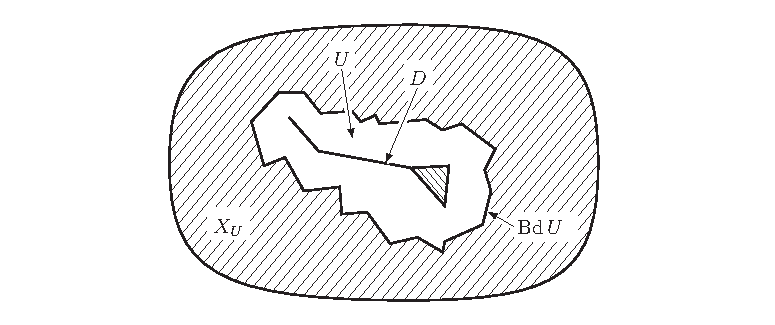
\includegraphics[width=.90\textwidth]{figures/8-12-4.pdf}
\caption*{图 8.12.4}
\end{figure}

在奇异理论中取复合
\[
H^k(X,D)\xleftarrow{i^*}H^k(X,\overline U)
\xrightarrow{k^*}H^k(X_U,\Bd U)
\xrightarrow{\frown\Gamma_U}H_{n-k}(X_U)
\xrightarrow{\ell_*}H_{n-k}(X\setminus D).
\]
其中 $k^*$ 为切除同构；$i^*,\ell_*$ 为同构，因为相应包含是同伦等价。以 $(i^*)^{-1}$ 开始的复合同构记为 $\lambda_{D,U}$。它不依赖所用具体剖分。

第三步：若 $A\subset E\subset D$，选取 $E$ 的合适邻域 $V\subset U$，则 $\lambda_{D,U}$ 与 $\lambda_{E,V}$ 和包含诱导映射交换。比较定义它们的两行复合，在中间插入
\[H^k(X_V,\overline U\setminus V),\qquad X_V=X\setminus V,\]
并用定向类 $\Gamma$ 在这个偶上的限制 $\Gamma'$ 作帽积。所有其余映射均为包含诱导；由帽积自然性，所组成的方块和三角形全部交换，因此得到所需关系。这里必须使用奇异群，因为 $U,V$ 可能不兼容同一个剖分，所插入的偶未必可三角剖分。

\sourcepage{517--518}
\begin{figure}[htbp]\centering
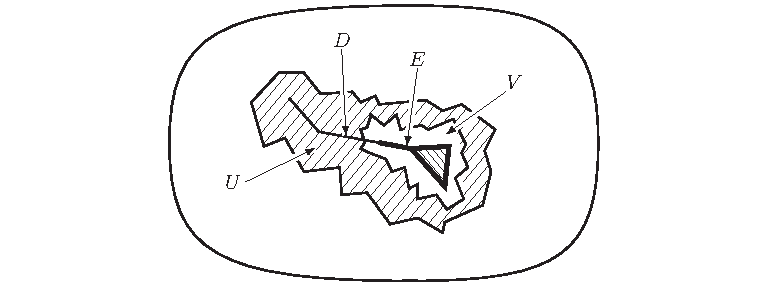
\includegraphics[width=.90\textwidth]{figures/8-12-5.pdf}
\caption*{图 8.12.5}
\end{figure}

第四步：令 $E=D$。对两个合适邻域 $U,U'$，可再选合适 $V\subset U\cap U'$，由第三步
\[\lambda_{D,U}=\lambda_{D,V}=\lambda_{D,U'}.\]
所以可定义 $\lambda_D$ 而不依赖邻域。其自然性同样由第三步得到。\hfill$\square$

\entry{推论}{8.12.7（Alexander 对偶）}固定 $n$，可以给每个 $S^n$ 中的非空真多面体 $A$ 指定同构
\[\alpha_A:\widetilde H^k(A)\to\widetilde H_{n-k-1}(S^n\setminus A),\]
且相对于包含自然。

\textbf{证明：}$k<n-1$ 时，取自然同构的复合 $\lambda_A\delta^*$。$k=n-1$ 时，使用上一节定义同构时的核及交换图，它们同样自然；$k=n$ 时平凡。\hfill$\square$

\subsection*{习题}
\begin{enumerate}
\item 设 $S^n$ 中多面体 $D$ 为不交集合 $A,B$ 的并，$A\approx S^k$，$B\approx S^{n-k-1}$，$0\le k\le n-1$。包含诱导
\[\varphi:\widetilde H_k(A)\to\widetilde H_k(S^n\setminus B),\qquad
\psi:\widetilde H_{n-k-1}(B)\to\widetilde H_{n-k-1}(S^n\setminus A).\]
由 Alexander 对偶，四个群都为无限循环群。证明两个映射差一个符号都是乘以同一整数 $m$。这个整数称为\emph{链环数}，衡量两个球面相互缠绕的次数（参见第 4.9 节习题 3）。〔提示：取剖分使 $A,B$ 满，且没有单形同时与二者相交。令 $C$ 为与 $A$ 不交的单形之并，比较 $B\subset C$ 所诱导的上同调映射及其自然 Alexander 对偶图。〕
\item 解释为什么图 8.12.2、8.12.3 各自实际上都是某个有序偶的“星形”。
\end{enumerate}
